\documentclass[a4paper]{article}

\usepackage[brazilian]{babel}
\usepackage[utf8]{inputenc}
\usepackage{amsfonts}
\usepackage{cite}
\usepackage{indentfirst}
\usepackage{amsmath}
\usepackage{tikz}
\usepackage{graphicx}
\usepackage[linesnumbered,lined,boxed,commentsnumbered]{algorithm2e}

\def\ok{\tikz\fill[scale=0.4](0,.35) -- (.25,0) -- (1,.7) -- (.25,.15) -- cycle;}

%\newcommand{\mod}[1]{\ \mathrm{mod}\ #1}

\title{Hashes Camaleão: Definição e Construção}
\author{Thiago Leucz Astrizi}

\begin{document}

\maketitle

\section{Introdução}

Hashes camaleão são funções muito semelhantes à hashes comuns. A
diferença é que elas possuem uma chave pública e uma chave privada
associada a elas. De posse de sua chave pública, é possível usá-las
para calcular o hash de algum dado qualquer, o que também permite
conferir se o cálculo de um hash está correto. Todas as propriedades
características à funções hash criptográficas (resistência à
pré-imagem, resistência à segunda pré-imagem, resistência à colisão)
estão presentes nas hashes camaleão quando elas são usadas somente
junto à sua chave pública.

Tendo acesso à chave privada de uma hash camaleão, a propriedade de
resistência à segunda pré-imagem se perde, o que também acaba com a
propriedade de resistência à colisões. Dependendo da construção da
hash camaleão, a propriedade de resistência à primeira pré-imagem
também pdode se perder quando tem-se acesso à chave privada.


\section{Hashes Camaleão Simples}

Um Esquema de Hash Camaleão Simples $CH$ é uma tupla formada por três
algoritmos eficientes $KeyGen$, $Hash$ e $Collision$ tais que:

\begin{itemize}
\item\textbf{KeyGen} é um algoritmo probabilístico invocado como
  $(\mathcal{PK}, \mathcal{SK}) \leftarrow^\$ KeyGen()$ onde
  $\mathcal{PK}$ é chamado de chave pública e $\mathcal{SK}$ é chamado
  de chave privada.
\item\textbf{Hash}: é um algoritmo determinístico invocado como $c
  \leftarrow Hash(\mathcal{PK}, m, r)$ onde $\mathcal{PK}$ é uma chave
  pública (como retornada por $KeyGen$), $m$ é uma mensagem, $r$ é um
  parâmetro aleatório e $c$ é o resumo criptográfico.
\item\textbf{Collision}: é um algoritmo probabilístico invocado como
  $r' \leftarrow^\$ Collision(\mathcal{SK}, m, r, m')$ onde
  $\mathcal{SK}$ é a chave privada (como retornada por $KeyGen$), $m$
  e $m'$ são duas mensagens distintas, $r$ é um parâmetro aleatório e
  $r'$ retornado é um valor tal que:

  $$ Hash(\mathcal{PK}, m,r) = Hash(\mathcal{PK}, m', r')$$
\item Assumimos que as mensagens pertencem à um espaço de mensagens
  finito $M$, os parâmetros aleatórios pertencem à um espaço de
  parâmetros aleatórios finito $R$ e todos os resumos criptográficos
  possíveis pertencem ao espaço re resumo criptográfico finito $C$.
  Dizemos que $CH=(KeyGen, Hash, Collision)$ é definida sobre $(M, R,
  C)$.
\end{itemize}

Podemos avaliar o quão seguros são vários tipos de esquemas de hash
camaleão observando as seguintes propriedades deles:

\begin{itemize}
\item\textbf{Resistência a Colisão: }Para todo adversário eficiente
  $\mathcal{A}$ a probabilidade do experimento abaixo retornar 1 é
  negligível:

  \noindent
  \begin{algorithm}[H]
    \SetAlgoLined
    \SetKwInOut{Input}{Entrada}\SetKwInOut{Output}{Saída}
    \SetKwFunction{FMain}{CollRes$_\mathcal{A}^{CH}$}
    \SetKwProg{Fn}{Experimento}{:}{} \Fn{\FMain{$n$}}{
      $(\mathcal{PK}, \mathcal{SK}) \leftarrow^\$
      $\textbf{KeyGen}($1^n$)\; $(m, r, m', r') \leftarrow
      \mathcal{A}(\mathcal{PK})$\; {\eIf{$Hash(\mathcal{PK}, m, r) =
          Hash(\mathcal{PK}, m', r')$ \textbf{e} $(m, r) \neq (m',
          r')$} {\textbf{retorne} 1\;} {\textbf{retorne} 0\;} } }\textbf{Fim}
  \end{algorithm}
  
\item\textbf{Resistência à Pré-Imagem: }Para todo adversário eficiente
  $\mathcal{A}$, a probabilidade do experimento abaixo retornar 1 é
  negligível:

  \noindent
  \begin{algorithm}[H]
    \SetAlgoLined
    \SetKwInOut{Input}{Entrada}\SetKwInOut{Output}{Saída}
    \SetKwFunction{FMain}{PreImg$_\mathcal{A}^{CH}$}
    \SetKwProg{Fn}{Experimento}{:}{} \Fn{\FMain{$n$}}{
      $(\mathcal{PK}, \mathcal{SK}) \leftarrow^\$$\textbf{KeyGen}($1^n$)\;
      $m \leftarrow^\$ M$\;
      $r \leftarrow^\$ R$\;
      $c \leftarrow Hash(\mathcal{PK}, m, r)$\;
      $m' \leftarrow \mathcal{A}(\mathcal{PK}, c, r)$\;
      {\eIf{$m' = m$}
        {\textbf{retorne} 1\;}
        {\textbf{retorne} 0\;}
      }
    }
    \textbf{Fim}
  \end{algorithm}

\item\textbf{Segurança Semântica: }Se para todo adversário eficiente
  $\mathcal{A}$, a probabilidade do experimento abaixo retornar 1 é
  negligível:

  \noindent
  \begin{algorithm}[H]
    \SetAlgoLined
    \SetKwInOut{Input}{Entrada}\SetKwInOut{Output}{Saída}
    \SetKwFunction{FMain}{SemanticSecurity$_\mathcal{A}^{CH}$}
    \SetKwProg{Fn}{Experimento}{:}{} \Fn{\FMain{$n$}}{
      $(\mathcal{PK},\mathcal{SK}) \leftarrow$\textbf{KeyGen}($1^n$)\;
      $(m_0, m_1) \leftarrow \mathcal{A}(\mathcal{PK})$\;
      $b \leftarrow^\$ \{0, 1\}$\;
      $r \leftarrow^\$ R$\;
      $c \leftarrow Hash(\mathcal{PK}, m_b)$\;
      $b' \leftarrow \mathcal{A}(c, r)$\;
      {\eIf{$b' = b$} {\textbf{retorne} 1\;} {\textbf{retorne} 0\;} } 
    }
  \end{algorithm}

  A segurança semântica implica a resistência à pré-imagem. Se um
  adversário pode calcular a pré-imagem com probabilidade
  não-negligível, então ele pode ser usado para construir um
  adversário que quebra a segurança semântica obtendo a pré-imagem do 
  
\item\textbf{Livre de Exposição de Chave:} Se para todo adversário
  eficiente $\mathcal{A}$, capaz de realizar uma quantidade polinomial
  de consultas à um oráculo que retorna colisões aleatórias no esquema
  de hash camaleão, a probabilidade do experimento abaixo retornar 1 é
  negligível.

\noindent
  \begin{algorithm}[H]
    \SetAlgoLined
    \SetKwInOut{Input}{Entrada}\SetKwInOut{Output}{Saída}
    \SetKwFunction{FMain}{KeyExposition$_\mathcal{A}^{CH}$}
    \SetKwProg{Fn}{Experimento}{:}{} \Fn{\FMain{$n$}}{
      $(\mathcal{PK}, \mathcal{SK}) \leftarrow$ \textbf{KeyGen}($1^n$)\;
      $\mathcal{SK'} \leftarrow \mathcal{A}^{Collision(\mathcal{SK},
        ., ., .)}(\mathcal{PK})$\;
      {\eIf{$\mathcal{SK} =
          \mathcal{SK'}$} {\textbf{retorne} 1\;} {\textbf{retorne}
          0\;} } }\textbf{Fim}
  \end{algorithm}

  Se um esquema de hash camaleão é livre de exposição de chaves, a
  mesma chave pode ser reutilizada mesmo quando colisões obtidas com a
  sua chave privada tornam-se públicas.
  
\item A \textbf{Resistência à Falsificação} afirma que para todo algoritmo
  adversário $\mathcal{A}$ que recebe uma chave pública $\mathcal{PK}$
  e pode consultar um número polinomial de vezes um oráculo que
  retorna diferentes resultados de $Collision(\mathcal{SK}, m, r, m')$
  para quaisquer valores de $m$, $r$ e $m'$, a probabilidade do
  experimento abaixo retornar 1 é negligível:

  \noindent
  \begin{algorithm}[H]
    \SetAlgoLined
    \SetKwInOut{Input}{Entrada}\SetKwInOut{Output}{Saída}
    \SetKwFunction{FMain}{ForgeRes$_\mathcal{A}^{CH}$}
    \SetKwProg{Fn}{Experimento}{:}{} \Fn{\FMain{$n$}}{ $(\mathcal{PK},
      \mathcal{SK}) \leftarrow$ \textbf{KeyGen}($1^n$)\; $(m, r, m',
      r') \leftarrow \mathcal{A}^{Collision(\mathcal{SK}, ., .,
        .)}(\mathcal{PK})$\; {\eIf{$Hash(\mathcal{PK}, m, r) =
          Hash(\mathcal{PK}, m', r')$ \textbf{e} $(m, r) \neq (m',
          r')$ \textbf{e} $r$ e $r'$ não foram retornados pelo
          oráculo} {\textbf{retorne} 1\;} {\textbf{retorne} 0\;} }
    }\textbf{Fim}
  \end{algorithm}

  Sem esta propriedade, uma vez que uma colisão é descoberta para uma
  mensagem $m$, não é possível garantir a segurança de qualquer outro
  uso da hash camaleão para calcular novamente o hash desta mesma
  mensagem. Contudo, a função ainda pode ser utilizada com a mesma
  chave para calcular o hash de outras mensagens. Na maioria dos casos
  esta propriedade é desejável, mas existem alguns usos de hash
  camaleão, como no caso das assinaturas camaleão como propostas por
  Krawczyk em \cite{krawczyk} nos quais a ausência desta propriedade é
  um requisito.

  É importante notar que a Resistência à Falsificação implica que um
  esquema é Livre de Exposição de Chaves. Afinal, um adversário capaz
  de computar eficientemente com probabilidade não-negligível a chave
  privada tendo acesso à um número polinomial de colisões pode ser
  usado para construir um adversário com uma vantagem não-negligível
  em encontrar colisões. Também será válida a contrapositiva de que se
  um esquema não é livre de exposição de chave, ele não será
  resistente à falsificação.
\item Um \textbf{Trapdoor de Pré-Imagem} é característica de algumas
  hashes camaleão onde de posse da chave privada podemos calcular não
  apenas uma colisão, mas também obter uma pré-imagem. Em outras
  palavras, existe um algoritmo probabilístico $PreImage(m, c)$ que
  retorna um valor $r$ tal que $Hash(m, r)=c$.

  Quando tal algoritmo existe, podemos apenas definir ele sem definir
  explicitamente o algoritmo que calcula colisões por meio da chave
  privada. Isso porque:

  $$Collision(\mathcal{SK}, m, r, m') = PreImage(\mathcal{SK}, m',
  Hash(\mathcal{PK}, m, r))$$
\end{itemize}

  
É importante notar que a composição de uma hash convencional e uma
hash camaleão é uma hash camaleão. Grande parte das definições de hash
camaleão assume que a mensagem de entrada possui um tamanho fixo ou
está em um formato pré-estabelecido. Em tais casos, assumimos que a
mensagem já passou previamente por uma função hash que a deixou no
formato adequado.

Uma função de hash camaleão $Hash(\mathcal{PK}, m, r)$ pode ser vista
como um caso particular de uma função hash com chave
$H_{\mathcal{PK}}(m||r)$ e deste fato podemos derivar algumas
propriedades. Se $|M||R| \geq s |T|$ para algum $s$ super-polinomial
em relação ao parâmetro de segurança $n$, então se a função hash é
resistente à colisão, então ela será uma função de mão única. Em tais
casos, a existência de uma função $PreImage$ também implica a
existência de uma função $Collision$ dada a chave privada.

\subsection{Construção Baseada em Permutações de Resíduos Qua\-drá\-ti\-cos
  (Krawczyk) (2000) \cite{krawczyk}}

\subsubsection{Funções}

\textbf{KeyGen: }Como chave pública, gere duas funções de permutação
que atuam sobre um mesmo Domínio. Chamaremos elas de $f_0$ e
$f_1$. Como chave privada, armazene o inverso destas funções:
$f_0^{-1}$ e $f_1^{-1}$.

A construção de Krawczyk usa como funções: $f_0(x) = x^2 \mod n$ e
$f_1(x) = 4x^2 \mod n$ para $n$ sendo um múltiplo de dois primos
grandes $p$ e $q$, tal que $p \equiv 3 \mod 8$ e $q \equiv 7 \mod
8$. E sendo a função definida apenas para resíduos quadráticos módulo
$n$ que também são primos em relação à $n$. A chave pública precisa
então apenas armazenar $n$ e a chave privada armazena $p$ e $q$. As
funções inversas envolvem raíz quadrada modular, as quais só sabemos
como resolver eficientemente módulo $n$ quando conhecemos os fatores
de $n$.

\textbf{Hash:} A função aceita como parâmetro aleatório somente
valores de $r$ que são resíduos quadráticos módulo $n$. Em seguida,
usando a representação binária da mensagem $m$, percorremos em ordem
cada um dos bits em uma iteração. Inicialmente o valor do hash é
considerado como igual a $r$. Em cada bit da iteração atualizamos como
novo valor da hash o valor anterior passado para $f_0$ se o bit for 0
ou o valor anterior passado para $f_1$ se o bit for 1.

\textbf{PreImage:} Para obter um valor válido de $r$ para que a
mensagem $m$ tenha o hash $C$, comece com o valor inicial de $C$ e
percorra a representação binária de $m$ de trás pra frente. Toda vez
que encontrar um 0, aplique sobre o valor atual de $r$ a função
$f_0^{-1}$. Sempre que encontrar um 1, aplique $f_1^{-1}$. O valor
final é o $r$ desejado.

\textbf{Collision:} Basta escolher uma mensagem $m'$ qualquer que seja
diferente de $m$ e calcular usando a equação:

$Collision(\mathcal{SK}, m, r) = (m', PreImage(\mathcal{SK}, m',
Hash(\mathcal{PK}, m, r)))$

Isso funciona pelo fato de que toda mensagem neste esquema é capaz de
produzir qualquer $c \in C$, bastando que se mude o valor de $r$
utilizado no hash.

\subsubsection{A Exposição de Chave}

Se encontramos uma colisão nesta hash camaleão, temos duas mensagens
que à partir de algum momento em que iteramos sobre seus bits, obtemos
valores distintos $x$ e $y$ tais que:

$$
x^2 \equiv 4y^2 \pmod n
$$

O que nos leva a:

$$
x^2 - 4y^2 \equiv 0 \pmod n
$$

$$
(x+2y)(x-2y) \equiv 0 \pmod n
$$

Desta forma, conseguimos fatorar $n$ e ter acesso à chave privada
$\mathcal{SK}$.

O mesmo raciocínio também nos mostra que encontrar uma colisão sem
acesso à $\mathcal{SK}$ é tão difícil quanto fatorar números.

%\subsection{Propriedades}

%As seguintes propriedades são específicas da construção de Krawczyk. O
%uso de diferentes permutações pode mudar as propriedades.

%\textbf{Resistência a Colisão: }Sim se assumirmos que é difícil
%fatorar números.

%\textbf{Ocultação de Mensagem: }Sim, usando a função \textbf{IForge}
%definida acima.

%\textbf{Livre de Exposição de Chave: } Não.
  
%\textbf{Cálculo de Primeira Pré-Imagem: }Sim.

\subsubsection{Exemplo Didático}

Começamos escolhendo os valores $p=3$ e $q=7$, que tem a propriedade
desejada de serem respectivamente côngruos a 3 e 7 módulo
8. Multiplicamos estes números para obtermos $n = 21 = pq$. No módulo
21 obtemos 3 números que são resíduos quadráticos: 1, 4 e 16.

Com estes três valores diferentes, definimos a função $f_0(x)=x^2\mod
21$ e $f_1=4x^2\mod 21$:

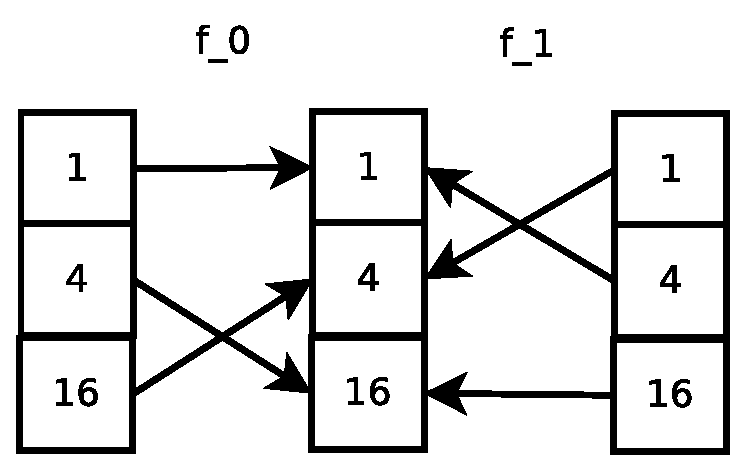
\includegraphics[width=5cm]{imagens/toy1.eps}

Para gerarmos o hash da mensagem com bits $01101$, geramos um $r$
aleatório que pode ser 1, 4 ou 16. No caso, escolhemos 4. Calculamos
então:

$$
f_1(f_0(f_1(f_1(f_0(4))))) = f_1(f_0(f_1(f_1(16)))) = f_1(f_0(f_1(16))) =
f_1(f_0(16)) = f_1(4) = 1
$$

Queremos que a mensagem com bits $00101$ tenha exatamente o mesmo hash
que a mensagem acima (no caso, 1). Para descobrirmos o valor de $r'$
que devemos associar à ela para este fim, calculamos:

$$
f_0^{-1}(f_0^{-1}(f_1^{-1}(f_0^{-1}(f_1^{-1}(1))))) =
f_0^{-1}(f_0^{-1}(f_1^{-1}(f_0^{-1}(4)))) =
f_0^{-1}(f_0^{-1}(f_1^{-1}(16))) =
$$
$$
=f_0^{-1}(f_0^{-1}(16)) = f_0^{-1}(4) = 16
$$

O que significa que podemos calcular o hash dessa mensagem e obteremos
$Hash(00101, 16)=1$. O que podemos conferir calculando abaixo:

$$
f_1(f_0(f_1(f_0(f_0(16))))) = f_1(f_0(f_1(f_0(4)))) = f_1(f_0(f_1(16))) =
f_1(f_0(16)) = f_1(4) = 1
$$

Exatamente o valor que era esperado.

\subsubsection{Medida de Desempenho}

Usando uma implementação em C baseada na biblioteca GNU MP com chaves
de 2048 bits e mensagens de 54 bytes, rodando em um computador Intel
i7, foi obtido os seguintes tempos de execução:

\begin{center}
\begin{tabular}{|c|c|c|c|c|c|}
  \hline
  KeyGen & 0,43400s & Hash & 0,00104s & Collision & 1,79000s\\
  \hline
\end{tabular}
\end{center}


\subsection{Construção Baseada em Logaritmo Discreto (Krawczyk) (2000)
  \cite{krawczyk}}

\subsubsection{Funções}

\textbf{KeyGen: }Primeiro encontre primos grandes $p$ e $q$ tais que
$p = kq+1$ e um grupo multiplicativo modular $\mathbb{Z}^{*}_p$ com um
gerador $g$.

A chave privada é um valor aleatório $x \in \mathbb{Z}^{*}_q$.

A chave pública é um valor $y = g^x \mod p$.

\textbf{Hash:}Dada uma mensagem $m \in \mathbb{Z}^{*}_q$ e um
parâmetro $r\in \mathbb{Z}^{*}_q$, a hash camaleão é obtida por meio
da definição:

$$
Hash(\mathcal{PK}=y, m, r) = g^my^r \mod p
$$

\textbf{PreImage:} Não. Seria necessário resolver o problema do
logaritmo discreto para implementar esta função.

\textbf{Collision:} A chave privada é o logaritmo discreto de $y$. Se
temos um $m$ e um $r$ que possui um hash conhecido e queremos que um
$m'$ qualquer gere o mesmo valor hash, o valor $r'$ necessário é
retornado por:

$$
Collision(\mathcal{SK}=x, m, r, m') = (m+xr-m')(x)^{-1}
$$

Este esquema não é livre de exposição de chaves. A chave secreta $x$
pode ser obtida por qualquer um que tenha acesso à uma colisão $(m,
r)$ e $(m', r')$ por meio da fórmula $m+xr = m'+xr'$.

%\subsection{Propriedades}

%\textbf{Resistência a Colisão: }Sim se assumirmos que é difícil
%calcular o logaritmo discreto no grupo escolhido.

%\textbf{Ocultação de Mensagem: }Sim, usando a função \textbf{IForge}.

%\textbf{Livre de Exposição de Chave: } Não.
  
%\textbf{Cálculo de Primeira Pré-Imagem: }Não.

\subsubsection{Exemplo Didático}

Vamos escolher um $p=11=(5)(2)+1$ com um $q=5$. Para o nosso valor de
$p$ temos então o seguinte grupo multiplicativo:

\begin{tabular}{|c||c|c|c|c|c|c|c|c|c|c|}
  \hline
$\times$&1&2&3&4&5&6&7&8&9&10\\
  \hline
  \hline
1&1&2&3&4&5&6&7&8&9&10\\
\hline
2&2&4&6&8&10&1&3&5&7&9\\
\hline
3&3&6&9&1&4&7&10&2&5&8\\
\hline
4&4&8&1&5&9&2&6&10&3&7\\
\hline
5&5&10&4&9&3&8&2&7&1&6\\
\hline
6&6&1&7&2&8&3&9&4&10&5\\
\hline
7&7&3&10&6&2&9&5&1&8&4\\
\hline
8&8&5&2&10&7&4&1&9&6&3\\
\hline
9&9&7&5&3&1&10&8&6&4&2\\
\hline
10&10&9&8&7&6&5&4&3&2&1\\
\hline
\end{tabular}

Com relação à exponenciação, se fizermos o valor de cada linha abaixo
elevado ao valor da coluna obtemos a tabela:

\begin{tabular}{|c||c|c|c|c|c|c|c|c|c|c|}
  \hline
  $a^b$&1&2&3&4&5&6&7&8&9&10\\
  \hline
  \hline
1&1&1&1&1&1&1&1&1&1&1\\
\hline
2&2&4&8&5&10&9&7&3&6&1\\
\hline
3&3&9&5&4&1&3&9&5&4&1\\
\hline
4&4&5&9&3&1&4&5&9&3&1\\
\hline
5&5&3&4&9&1&5&3&4&9&1\\
\hline
6&6&3&7&9&10&5&8&4&2&1\\
\hline
7&7&5&2&3&10&4&6&9&8&1\\
\hline
8&8&9&6&4&10&3&2&5&7&1\\
\hline
9&9&4&3&5&1&9&4&3&5&1\\
\hline
10&10&1&10&1&10&1&10&1&10&1\\
\hline
\end{tabular}

Podemos escolher qualquer elemento cuja ordem é $q=5$ como
gerador. Pode ser o 3, 4, 5 ou 9. Escolheremos então $g=5$. Podemos
escolher como chave privada os valores 1, 2, 3 ou 4, pois eles tem
ordem $q=5$. Façamos então $\mathcal{SK}=3$. O que faz com que nossa
chave pública seja $\mathcal{PK}=5^3\mod 11 = 4$.

Vamos calcular um hash para a mensagem representada pelo número
$m=8$. O nosso parâmetro aleatório $r$ pode ser 1, 2, 3 ou 4. Façamos
então $r=2$. A hash é calculada então por:

$$
Hash(\mathcal{PK}=4, m=8, r=2) = g^my^r = 5^84^2 \mod 11 = 9
$$

Agora supondo que tenhamos a chave privada, queremos fazer com que a
mensagem $m'=7$ tenha exatamente o mesmo valor de hash. Para isso
fazemos:

\begin{equation}
\begin{split}
  UForge(\mathcal{SK}=3, m=8, r=2, m'=7) &= \frac{m+xr-m'}{x} \mod 5\\
  &= 2(3)^{-1} \mod 5 = (2)(2) \mod 5 = 4
\end{split}
\end{equation}

Para checar que isso é correto, vamos calcular:

$$ Hash(\mathcal{PK}=4, m'=7, r'=4) = g^{m'}y^{r'} = 5^74^4 \mod 11 =
(3)(3)= 9
$$

Exatamente o resultado esperado.

\subsubsection{Medida de Desempenho}

\begin{center}
\begin{tabular}{|c|c|c|c|c|c|}
  \hline
  KeyGen & 0,005490s & Hash & 0,009530s & Collision & 0,000032s\\
  \hline
\end{tabular}
\end{center}

\subsection{Construção Baseada em Assinaturas  Nyberg-Rueppel
  (Ateniese e Medeiros) (2005)\cite{ateniese}}

Esta construção se baseia na existência do esquema de assinaturas
Nyberg-Rueppel, um dos esquemas baseados no ElGamal. Nele, começamos
gerando dois números primos $p$ e $q$ tais que $p=2q+1$. Escolhemos
também um gerador $g$ do subgrupo de resíduos quadráticos de
$\mathbb{Z}_p$ de ordem $q$. Escolhemos como chave privada um número
$x$ módulo $q$ e escolhemos como chave pública um valor $y=g^x \mod
p$.

Em uma das variações dessa assinatura, assinar uma mensagem $m$ é
feito por meio da equação:

$$
Sign(m) = (r, s) = ((g^k \mod p) \mod q, k-rmx \mod q)
$$

E uma assinatura $(r, s)$ é válida para uma mensagem $m$ se:

$$
r = (g^sy^{rm} \mod p) \mod q
$$

O valor $k$ acima deve ser sempre escolhido aleatoriamente e não pode
ser revelado, ou a chave privada poderia ser facilmente extraída.

A ideia será gerar um esquema de hash camaleão no qual a equação de
verificação acima será usada para o nosso hash e a equação de
assinatura será usada para obter uma pré-imagem após fazermos algumas
modificações. A única mudança que precisará ser feita será a
substituição do produto $mr$ pelo resultado do hash convencional
$\mathcal{H}(m||r)$ em todas as equações acima. Desta forma, ficaremos
com as equações abaixo que servirão de base para nosso hash camaleão.

Equações de verificação:

$$
r = (g^k \mod p) \mod q
$$

$$
s = k-\mathcal{H}(m||r)x \mod q
$$

Equação de assinatura:

$$
r = (g^sy^{\mathcal{H}(m||r)} \mod p) \mod q
$$

\textbf{A Compreender: }Por que foi necessário fazer a substituição de
$mr$ por $\mathcal{H}(m||r)$? A rigor, o esquema continuaria
funcionando se essa substituição não tivesse sido feita.

\subsubsection{Funções}

\textbf{KeyGen: }A geração de chaves é idêntica à do esquema de
assinatura. Começamos gerando dois números primos $p$ e $q$ tais que
$p=2q+1$. Escolhemos também um gerador $g$ do subgrupo de resíduos
quadráticos de $\mathbb{Z}_p$ de ordem $q$. Escolhemos como chave
privada um número $x$ módulo $q$ e escolhemos como chave pública um
valor $y=g^x \mod p$.

\textbf{Hash: } Geraremos uma função de hash que será baseada na
verificação para saber se uma assinatura Nyberg-Rueppel é válida para
uma mensagem $m$. Nosso hash será definido como:

$$
Hash(m, (r, s)) = r - (g^sy^{\mathcal{H}(m, r)} \mod p) \mod q
$$

A função hash pode então ser interpretada intuitivamente como uma
forma de calcular a diferença entre o parâmetro aleatório $(r, s)$ e
uma assinatura legítima de Nyberg-Rueppel. Se por uma grande
coincidência escolhêssemos como valores $(r, s)$ uma assinatura
Nyberg-Rueppel legítima da mensagem $m$, então isso significa que o
valor de nosso hash seria zero. Nos demais casos, o hash assume
qualquer outro valor módulo $q$.


\textbf{PreImage:} Se a nossa função hash pode ser vista
intuitivamente como a diferença entre o parâmetro aleatório $(r, s)$ e
uma assinatura legítima, então a nossa função de pré-imagem pode ser
vista como um método que calcula uma assinatura legítima
Nyberg-Rueppel e depois adiciona uma perturbação na assinatura para
que ela fique com a diferença desejada em relação à uma assinatura legítima.

Dada uma mensagem $m$ e o \textit{digest} desejado $c$, podemos gerar
um valor $(r, s)$ fazendo:

$$
r = c + (g^k \mod p) \mod q
$$

$$
s = k-\mathcal{H}(m||r)x \mod q
$$

\textbf{Prova: }Demonstraremos que $Hash(m, PreImage(c, m)) = c$.

\begin{equation*}
  \begin{split}
    &Hash(m, PreImage(c, m))\\
    &= Hash(m, (c+(g^k \mod p) \mod q, k-x\mathcal{H}(m, r) \mod q))\\
    &= r - (g^sy^{\mathcal{H}(m, r)} \mod p) \mod q\\
    &= r - (g^{x\mathcal{H}(m, r) + s} \mod p) \mod q\\
    &= r - (g^{x\mathcal{H}(m, r) + k - x\mathcal{H}(m, r)} \mod p) \mod q\\
    &= c+ (g^k \mod p) - (g^{k} \mod p) \mod q\\
    &= c\\
  \end{split}
\end{equation*}



\textbf{Collision:} Como existe uma função $PreImage$, podemos
obter uma colisão calculando:

$$ Collision(\mathcal{Sk}, m, r, m') = PreImage(\mathcal{SK},
Hash(\mathcal{PK}, m, r), m')
$$

\subsubsection{Variações}

Ateniese e Medeiros, no mesmo artigo em que apresentou esta construção,
apontou que é possível definir a função hash como:

$$ Hash(\mathcal{PK}, m, (r, s)) =
\left(ry^{\mathcal{H}(m||r)}g^{s} \right)\mod p
$$

Em tal caso, para obter a função $PreImage$, calculamos:

$$
r'=Cg^{-k} \mod p
$$

$$
s' = k-\mathcal{H}(m||r')x \mod q
$$

Pode-se provar que isso também funciona mostrando que $Hash(m,
PreImage(m, c))=c$:

\begin{equation}
\begin{split}
  Hash(m, PreImage(m, c))
  &= Hash(m, (cg^{-k} \mod p, k-\mathcal{H}(m||r)x \mod q))\\
  &= (cg^{-k} \mod p)y^{\mathcal{H}(m||r)}g^{k-\mathcal{H}(m||r)x\mod q}\mod p\\
  &= (cg^{-k} \mod p)g^{\mathcal{H}(m||r)x}g^{k-\mathcal{H}(m||r)x\mod q}\mod p\\
  &= cg^{-k+\mathcal{H}(m||r)x+k-\mathcal{H}(m||r)x \mod q} \mod p\\
  &= c\\
\end{split}
\end{equation}

O artigo que introduz a assinatura de Nyberg-Rueppel \cite{nyberg}
menciona um total de 5 variações de cálculo de assinatura e
verificação que podem ser adaptados para esquemas de hash camaleão
bastante semelhantes. A imagem abaixo retirada do artigo apresdenta
todas as variações:

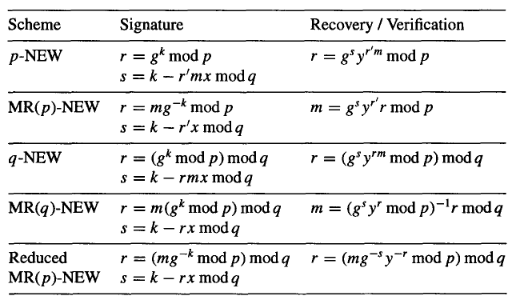
\includegraphics[width=\textwidth]{imagens/nyberg.png}

Todas as variações acima foram geradas à partir do mesmo conjunto
inicial de equações e por isso são relacionados.

O q-NEW foi o primeiro esquema que mostramos e mostra-se o mais
atrativo por não precisar de qualquer cálculo de inverso
multiplicativo. O p-NEW é quase igual, sendo que a principal diferença
é em qual momento calculamos o módulo $q$ do $r$ ($r'=r \mod q$).

O MR(p)-NEW é a variação que vimos logo depois e que também foi
apresentada por Ateniese e Medeiros na forma adaptada de um hash
camaleão.

Podemos mostrar aqui também como seria um hash camaleão baseado na
forma MR(q)-NEW e Reduced MR(p)-NEW.

O hash camaleão MR(q)-NEW seria:

$$
Hash(m, (r, s)) = (g^sy^{\mathcal{H}(m||r) \mod p})^{-1}r \mod q
$$
$$
PreImage(c, m) = (c(g^k \mod p) \mod q, k-\mathcal{H}(m||r)x \mod q)
$$

\textbf{Prova: }Demonstraremos que $Hash(m, PreImage(c, m)) = c$.

\begin{equation*}
  \begin{split}
    &Hash(m, PreImage(c, m))\\
    &= Hash(m, (cg^{k} \mod p, k-x\mathcal{H}(m||r) \mod q))\\
    &= (g^sy^{\mathcal{H}(m||r)})^{-1}r \mod p\\
    &= (g^{s+x\mathcal{H}(m||r)})^{-1}r \mod p\\
    &= (g^{k-x\mathcal{H}(m||r)+x\mathcal{H}(m||r)})^{-1}r \mod p\\
    &= g^{-k}cg^{k} \mod p\\
    &= c\\
  \end{split}
\end{equation*}

Por fim, o hash camaleão Reduced MR(p)-NEW seria:

$$
Hash(m, (r, s)) = r-(mg^{-s}y^{-r} \mod p) \mod q
$$

$$
PreImage(c, m) = (c+(mg^{-k} \mod p) \mod q, k-rx \mod q)
$$

\textbf{Prova: }Demonstraremos que $Hash(m, PreImage(c, m)) = c$.

\begin{equation*}
  \begin{split}
    &Hash(m, PreImage(c, m))\\
    &= Hash(m, (c+(mg^{-k} \mod p) \mod q, k-rx \mod q))\\
    &= r-(mg^{-s}y^{-r} \mod p) \mod q\\
    &= r-(mg^{-s-xr} \mod p) \mod q\\
    &= r-(mg^{-k+rx-xr} \mod p) \mod q\\
    &= r-(mg^{-k} \mod p) \mod q\\
    &= c+(mg^{-k} \mod p)-(mg^{-k} \mod p) \mod q\\
    &= c\\
  \end{split}
\end{equation*}

\subsubsection{Segurança}

Uma das vantagens de definir hashes camaleão à partir de assinaturas
digitais é que se as assinaturas são seguras, pode-se derivar deste
fato muito da segurança das hashes camaleão baseadas nelas.

A resistência à colisão e o fato do esquema ser livre de exposição de
chave deriva da própria segurança da assinatura de Nyber Rueppel.

Contudo, não necessariamente um esquema de assinatura continua sendo
seguro se uma mesma mensagem é assinada várias vezes e um atacante tem
acesso à tais assinaturas. Felizmente, no caso da assinatura de
Nyberg-Rueppel, isso foi demonstrado em \cite{twin}, no Apêndice A.

Já a segurança semântica deste esquema foi demonstrada por Ateniese e
Medeiros no artigo que apresentou este esquema de assinatura.

\subsubsection{Medida de Desempenho}

Este é o desempenho obtido do hash camaleão de Nyberg-Rueppel q-NEW,
apresentado por Ateniese e Medeiros e que mostra-se mais atrativo por
não precisar de cálculo de inverso multiplicativo:

\begin{center}
\begin{tabular}{|c|c|c|c|c|c|}
  \hline
  KeyGen & 0,017544s & Hash & 0,019996s & Collision & 0,007057s\\
  \hline
\end{tabular}
\end{center}

\subsection{Construção Baseada no DSA}

A seção anterior nos leva a questionar se a mesma técnica não poderia
ser usada para obter hashes camaleão baseados em outras assinaturas
que também seriam derivadas do Elgamal. Seria uma questão de montar um
hash à partir da equação de verificação e obter uma função de
pré-imagem à partir da equação que define a assinatura.

Esta seção mostra que é possível fazer isso com a assinatura DSA.

\subsubsection{Funções}

\textbf{KeyGen: } A geração de chaves funciona de maneira idêntica à
geração do DSA. Primeiro escolhe-se dois primos $p$ e $q$ tal que
$p-1$ é um múltiplo de $q$. Escolhemos então um inteiro $h$ aleatório
entre 2 e $p-2$. É possível simplesmente usar $h=2$. Por fim,
computamos $g=h^{(p-1)/q} \mod p$. Assim $(p, q, g)$ são os parâmetros
de sistema usados pelo algoritmo.

Para a chave privada escolhemos um valor $\mathcal{SK}=x$ menor que
$q$. E a chave pública é $\mathcal{PK}=y=g^x \mod p$;

\textbf{Hash:}

Verificar uma assinatura DSA $(r, s)$ para uma mensagem $m$ envolve
checar se é verdade que:

$$
(g^{\frac{\mathcal{H}(m)}{s} \mod q}y^{\frac{r}{s} \mod q} \mod p) \mod q = r
$$

Baseando-se nessa equação construímos nossa função de hash:

$$
Hash(m, (r, s)) = r - (g^{\frac{\mathcal{H}(m)}{s} \mod q}y^{\frac{r}{s} \mod q} \mod p) \mod q
$$

\textbf{PreImage:}

Criar uma assinatura legítima DSA para a mensagem $m$ envolve escolher
$(r, s)$ tais que:

$$
r = (g^k \mod p) \mod q
$$

$$
s = k^{-1}(\mathcal{H}(m)+xr) \mod q)
$$

Exatamente como na primeira assinatura Nyberg-Rueppel da seção
anteriror, podemos controlar o valor da hash que definimos aqui apenas
perturbando o valor de $r$ somando à ele o valor do \textit{digest}
desejado:

$$
PreImage(m, c) = (c + (g^k \mod p) \mod q,k^{-1}(\mathcal{H}(m)+xr) \mod q)
$$

\textbf{Prova:}Demonstraremos que $Hash(m, PreImage(c, m)) = c$.

\begin{equation*}
  \begin{split}
    &Hash(m, PreImage(c, m))\\
    &= Hash(m, (c + (g^k \mod p) \mod q, k^{-1}(\mathcal{H}(m)+xr) \mod q))\\
    &= r - (g^{\frac{\mathcal{H}(m)}{s} \mod q}y^{\frac{r}{s} \mod q} \mod p) \mod q\\
    &= r - (g^{\frac{\mathcal{H}(m)+xr}{s} \mod q} \mod p) \mod q\\
    &= r - (g^{\frac{k(\mathcal{H}(m)+xr)}{\mathcal{H}(m)+xr} \mod q} \mod p) \mod q\\
    &= c + (g^k \mod p) - (g^{k} \mod p) \mod q\\
    &= c\\
    \end{split}
\end{equation*}

\subsubsection{Segurança}

Assim como na seção anterior, a segurança deste esquema deriva da
própria segurança do esquema de assinaturas DSA e da propriedade que o
DSA continua seguro mesmo que um atacante tenha acesso a mais de uma
assinatura válida para uma mesma mensagem. A segunda propriedade foi
demonstrada em \cite{twin}.

A segurança semântica deste esquema ainda está para ser demonstrada.

\subsubsection{Medida de Desempenho}

\begin{center}
\begin{tabular}{|c|c|c|c|c|c|}
  \hline
  KeyGen & 0,0020026s & Hash & 0,018312s & Collision & 0,006846s\\
  \hline
\end{tabular}
\end{center}


\subsection{Construção Baseada no Protocolo Sigma de Fiat-Shamir
  (Mihir Bellare e Todor Ristov) (2008)\cite{sigma}}

Esta construção foi obtida em um artigo no qual os autores estavam
demonstrando a possibilidade de construir novas funções hash com
provas de segurança à partir de protocolos sigma. Eles demonstraram
que as funções hash que eles obtiveram também tinham a propriedade de
ser hashes camaleão.

\subsubsection{Funções}

\textbf{KeyGen: } Gere dois primos aleatórios $p$ e $q$. Faça $n=pq$.

Como chave pública, gere um vetor $s$ de $k$ números que sejam
resíduos quadráticos módulo $n$, sendo $k$ o número de bits das
mensagens a serem recebidas. Para adotar as melhorias propostas no
Protocolo Micali-Shamir, tais números devem ser primos pequenos que
sejam resíduos quadráticos módulo $n$, Adicione também à chave o valor
$n$.

Como chave privada, gere um vetor $v$ de $k$ números tal que
$v_i=s_i^{-2} \mod n$ e também adicione à chave os fatores $p$ e $q$.

\textbf{Hash: } Seja a mensagem $m$ um vetor binário com $k$ bits e
sendo $r \leq n/2$, a hash é obtida por:

$$ Hash(\mathcal{PK}, m, r) = r^2\prod_{m_i=1}v_i \mod n
$$

\textbf{PreImage: } Esta função é definida como:

$$
PreImage(\mathcal{SK}, C, m') = \sqrt{C}\prod_{m'_i=1}s_i \mod n
$$

A raíz quadrada modular só pode ser calculada por quem conheça os
fatores primos de $n$. A fórmula acima funciona, pois:

$$ C = r^2\prod_{m_i=1}v_i =
r^2\prod_{m_i=1}\frac{1}{s_i^2}\Longrightarrow r=\sqrt{C}\prod_{m'_i=1}s_i
$$

\subsubsection{O Problema da Exposição de Chave}

Esta construção não é livre de exposição de chave. Se somos capazes de
obter uma colisão na qual as duas mensagens que colidem possuem bits
1s nas mesmas posições, para cada bit 1 em comum, podemos gerar uma
nova colisão para novas mensagens idênticas, mas que possuem o bit 1
correspondente trocado para 0, mantendo os parâmetros aleatórios das
mensagens idênticos.

Sendo assim, a probabilidade de que uma colisão não revele novas
colisões derivadas é negligível.

\subsubsection{Medida de Desempenho}

\begin{center}
\begin{tabular}{|c|c|c|c|c|c|}
  \hline
  KeyGen & 4,838347s & Hash & 0,000004s & Collision & 0,004199s\\
  \hline
\end{tabular}
\end{center}

\subsection{Construção Baseada no Protocolo Sigma de Okamoto
  (Mihir Bellare e Todor Ristov) (2008)\cite{sigma}}

Esta construção foi obtida assim como a anterior à partir de
protocolos sigma já existentes após o autor perceber a relação
existente entre protocolos sigma e hashes camaleão. Mas ao contrário
do método anterior, esta construção não se destaca por ter vantagem em
desempenho comparada à outras construções e nem tem a propriedade
desejável de ser livre de exposição de chave.

\subsubsection{Funções}

\textbf{KeyGen: } Obtenha um grupo onde calcular o logaritmo discreto
é um problema difícil. Escolha como chave pública $(g_1, g_2, x)$ onde
$g_1$ e $g_2$ são geradores e escolha como chave privada $(s_1, s_2)$
tais que $g_1^{s_1}g_2^{s_2} = x$.

\textbf{Hash: } É definida pela seguinte função:

$$
Hash(\mathcal{PK}=(g_1, g_2, x), m, r=(r_1, r_2)) = x^mg_1^{r_1}g_2^{r_2}
$$

\textbf{Collision: } Pela propriedade da exponenciação, dados $m$,
$m'$ e $r=(r_1, r_2)$ conhecidos, podemos obter $r'=(r_1', r_2')$ tal
que $Hash(\mathcal{PK}, m, r) = Hash(\mathcal{PK}, m', r')$ por meio
da equação:

$$
r_1' = (m-m')s_1+r_1
$$

$$
r_2' = (m-m')s_2+r_2
$$

A mesma equação também nos revela que o esquema não é livre da
exposição de chaves, pois diante de uma colisão os valores $s_1$,
$s_2$ podem ser trivialmente isolados.

\textbf{Prova: }Pode-seprovar o funcionamento desta construção
mostrando que $Hash(m', Collision(m, r, m')) = Hash(m, r)$:

\begin{equation}
\begin{split}
  Hash(m', Collision(m, r, m'))
  &= Hash(m', ((m-m')s_1+r_1, (m-m')s_2+r_2))\\
  &= x^{m'}g_1^{(m-m')s_1+r_1}g_2^{(m-m')s_2+r_2}\\
  &= x^{m'}x^{m-m'}g_1^{r_1}g_2^{r_2}\\
  &= Hash(m, r)\\
\end{split}
\end{equation}

Contudo, embora funcione, este esquema não apresenta qualquer vantagem
em relação à outros esquemas baseados em logaritmo discreto.

\subsection{Construção Baseada em Reticulados (David Cash)
  (2010)\cite{reticulado}}

A segurança deste esquema não se baseia em fatoração de números ou no
logaritmo discreto, mas no Problema da Solução Inteira Pequena (SIS),
um problema baseado em reticulados. Isso torna este esquema seguro
mesmo diante de computadores quânticos até onde se sabe.

A segurança desta construção se baseia no fato de que é difícil
encontrar qualquer vetor $x$ inteiro cuja norma euclideana é
suficientemente pequena tal que $Ax = b$, onde $A$ é uma matriz
inteira retangular suficientemente grande em termos de número de
colunas e $b$ é um vetor conhecido.

A construção utiliza sempre matrizes e vetores inteiros módulo $q$ nas
definições seguintes.

\subsubsection{Funções}

\textbf{Keygen:} Seja $H \in \mathbb{Z}^{n\times n}$ uma matriz
inversível qualquer, podendo ser uma matriz identidade e $G$ uma
matriz selecionada previamente tal que para $G$ é conhecido método
eficiente de obter valores de $x$ com norma euclideana pequena tais
que $Gx = b$.

Como chave privada, gere uma matriz aleatória $R \in \mathbb{Z}^{w
  \times n}$. Os valores dela devem ser pequenos para aumentar a
qualidade do \textit{trapdoor}.

Como chave pública gere a matriz $A=[\overline{A}|HG-\overline{A}R]$,
onde $\overline{A}$ é uma submatriz inteira gerada aleatoriamente.

O objetivo desta construção é que com isso geramos matrizes tais que:

$$
A\left[\begin{matrix}R\\I\end{matrix}\right] = HG
$$

\textbf{Hash: } Seja $\mathcal{H}$ uma função hash convencional tal
que a saída dela possa ser interpretada como um vetor inteiro módulo
$q$ com mesmo número de elementos que o número de linhas de
$A$. Definimos a função hash do esquema como:

$$
Hash(\mathcal{PK}=A, m, r) = \mathcal{H}(m) + Ar \mod q
$$

\textbf{Collision: } Como queremos encontrar uma colisão, dado $m$,
$r$ e $m'$, queremos encontrar um valor $r'$ de norma euclideana
pequena tal que:

$$
\mathcal{H}(m) + Ar  \equiv \mathcal{H}(m') + Ar' \pmod q
$$

O valor de $r'$ é então uma solução para a equação $Ax =
\mathcal{H}(m) - \mathcal{H}(m') + Ar \mod q$.

Par obter uma solução para esta equação utiliza-se um vetor qualquer
de norma euclideana pequena $p$ e obtém-se o valor $x'$ tal que ele
seja a solução para a equação abaixo:

$$
Gx' = H^{-1}(\mathcal{H}(m) - \mathcal{H}(m') + Ar - Ap) \mod q
$$

Dados os valores de $x'$ e $p$, a nossa função $Collision$ é definida
como:

$$ Collision(\mathcal{SK}=R, m, r, m') = p +
\left[\begin{matrix}R\\I\end{matrix}\right]x' \mod q
$$

\textbf{Prova:}

Para provar que o resultado obtido é correto, basta mostrarmos que o
valor retornado pela função acima é uma solução para $Ax =
\mathcal{H}(m) - \mathcal{H}(m') + Ar \mod q$. Se multiplicarmos o
resultado da função de colisão pela matriz $A$ obtemos:

$$ A(p+\left[\begin{matrix}R\\I\end{matrix}\right]x') = Ap +
A\left[\begin{matrix}R\\I\end{matrix}\right]x'\\
$$

Temos que $A\left[\begin{matrix}R\\I\end{matrix}\right] = HG$:

$$
Ap + A\left[\begin{matrix}R\\I\end{matrix}\right]x' = Ap + HGx'
$$

Sabemos também que $Gx' = H^{-1}(\mathcal{H}(m) - \mathcal{H}(m') + Ar
- Ap)$, e portanto:

$$
Ap + HGx' = Ap + H H^{-1}(\mathcal{H}(m) - \mathcal{H}(m') + Ar - Ap)
$$

Após multiplicar $H$ pela sua inversa e dos dis termos $Ap$ se
anularem, obtemos o resultado que queríamos para mostrar a corretude
da função de colisão.

\subsubsection{Detalhes da Construção}

Para garantir a segurança do esquema, o número de colunas da matriz
$A$ de $n$ linhas deve ser ao menos $n\log q$. Além disso, só devemos
considerar um vetor como tendo uma norma euclideana suficientemente
pequena para ser aceito como solução quando a norma dele é no máximo
um valor próximo de $\sqrt{n \log q}$.

\textbf{Construção da matriz G:}

Seja $q=2^k$. Seja o vetor $g=[1, 2, 4, 8, \ldots, 2^{k-1}]$. Podemos
construir a matriz $G$ então como:

$$
\left[\begin{matrix}
    g & \ldots & \ldots & \ldots\\
    \ldots & g & \ldots & \ldots\\
    \vdots & \vdots & \ddots & \vdots\\
    \ldots & \ldots & \ldots & g\\
  \end{matrix}\right]
$$

Desta forma, podemos encontrar uma solução para uma equação $Gx=u \mod
q$ simplesmente escolhendo $x$ como a representação binária de
$u$. Esta é uma forma viável de gerar vetores suficientemente pequenos
apenas quando temos uma construção com um valor muito pequeno de $n$.

Para os demias casos, o modo recomendado de obter uma solução é gerar
um reticulado com uma base formada pela matriz esparsa preenchida por
2 na diagonal e com um valor -1 abaixo de cada diagonal e obter um
vetor suficientemente pequeno por meio de algoritmos de amostragem
gaussiana.

\subsubsection{Medida de Desempenho}

\begin{center}
\begin{tabular}{|c|c|c|c|c|c|}
  \hline
  KeyGen & -- & Hash & 0,0017129s & Collision & --\\
  \hline
\end{tabular}
\end{center}

Também é importante mencionar que para valores consifderados seguros,
o tamanho da chave privada nesta construção chega a 613KB. A chave
pública é seis vezes menor e pode ser reduzida muito mais por meio das
mesmas técnicas utilizadas para reduzir tamanhos de chave de funções
hash baseados em reticulados.

\subsection{Características dos Esquemas Apresentados}

A tabela abaixo sintetiza as características mais relevantes dos
esquemas vistos nesta seção. Cada esquema está identificado pelo
número da subseção em que ele foi apresentado.

\begin{center}
  \begin{tabular}{|c|c|c|c|c|c|c|c|}
    \hline
    Esquema&2.1&2.2&2.3&2.4&2.5&2.6&2.7\\
    \hline
    Livre de Exposição de Chave&X&X&\ok&\ok&X&X&\ok\\
    \hline
    Resistência à Falsificação&X&X&\ok&\ok&X&X&\ok\\
    \hline
    Trapdoor de Pré-Imagem&\ok&X&\ok&\ok&\ok&X&X\\
    \hline
  \end{tabular}
\end{center}




\bibliography{report}{}\bibliographystyle{plain}
\end{document}
%%%%%%%%%%%%%%%%%%%%%%%%%%%%%%%%%%%%%%%%%%%%%%%%%%%%%%%%%%%%%%%%%

\section{Hashes Camaleão com ID}

\subsection{Construção Baseada no RSA (Ateniese e Medeiros) (2005)\cite{ateniese}}

Este esquema se baseia nas propriedades da assinatura e criptografia
RSA. Elas nos dizem que se temos dois primos grandes $p$ e $q$,
podemos obter um número primo em relação a $\phi(pq)$ que chamamos de
$e$ e o seu inverso multiplicativo módulo $\phi(pq)$, que chamamos de
$d$. Seja $n=pq$.

Temos então que $M'=M^e \mod n$ e $M=M'^d \mod n$. Tratamos $(e, n)$
como a chave pública e $(d, p, q)$ como a chave privada. As chaves
podem ser calculadas facilmente somente por alguém que conhece os
fatores primos que formam $n$.

\subsection{Funções}

\textbf{KeyGen: } Idêntica à geração de chaves do RSA. A chave pública
é $(e, n)$ e a chave privada é $(d, p, q)$. A única restrição
adicional é que $e$ deve ser um número primo, não apenas primo em
relação a $\phi(n)$.

\textbf{Hash: } Assuma que esta função além da mensagem $m$ e do
parâmetro $r$ recebe também um $\mathcal{L}$ que representa uma
identificação ou rótulo da operação sendo realizada. Seja $C$ e
$\mathcal{H}$ duas funções hash convencionais com um tamanho ajustado
de acordo com parâmetros de segurança e de modo que $\mathcal{H}$ gere
valores sempre menores que $e$.

Calculamos o hash camaleão calculandoda seguinte forma:

$$
Hash(\mathcal{L}, m, r) = C(\mathcal{L})^{\mathcal{H}(m)}r^e \mod n
$$

\textbf{PreImage:} Não está presente neste esquema.

\textbf{UForge:} Para obtermos um novo valor $r'$ para um dado $m'$
que tenha mesmo hash que $m$ e $r$, podemos comaçar pela equação:

$$
C(\mathcal{L})^{\mathcal{H}(m)}r^e \equiv C(\mathcal{L})^{\mathcal{H}(m')}r'^e \pmod n
$$

Dividindo ambos os lados da equação por $C(\mathcal{L})^{\mathcal{H}(m')}$:

$$
C(\mathcal{L})^{\mathcal{H}(m)-\mathcal{H}(m')}r^e \equiv r'^e \pmod n
$$

Fazendo a equação ser elevada ao expoente $d$ (que pertence à chave
privada):

$$
rC(\mathcal{L})^{d(\mathcal{H}(m)-\mathcal{H}(m'))} \equiv r' \pmod n
$$

E portanto, podemos calcular $r'$ por meio de \textbf{UForge} com a
equação abaixo:

$$
r' = rC(\mathcal{L})^{d(\mathcal{H}(m)-\mathcal{H}(m'))} \mod n
$$

\textbf{iForge:} É possível extrair o valor $C(\mathcal{L})^d$ por
meio de uma colisão, que representa uma assinatura RSA sobre o valor
$\mathcal{L}$. Obtendo este valor, pode-se criar qualquer outra
colisão neste esquema de hash, mesmo sem sermos capazes de obter a
chave privada $d$.

O modo de obter $C(\mathcal{L})^d$ é à partir das equações
acima. Temos inicialmente que:

$$
r'/r \equiv C(\mathcal{L})^{d(\mathcal{H}(m)-\mathcal{H}(m'))} \pmod n
$$

Como $e$ é primo e maior que qualquer valor retornado por
$\mathcal{H}$, então $mdc(e, \mathcal{H}(m)-\mathcal{H}(m')) = 1$. E
portanto, usando o Algoritmo Estendido de Euclides, podemos obter
valores $\alpha$ e $\beta$ tais que
$\alpha(\mathcal{H}(m)-\mathcal{H}(m'))+\beta e = 1$.

Elevando os dois lados da equação acima por $\alpha$ ficamos com:

$$
(r'/r)^\alpha \equiv C(\mathcal{L})^{d(\mathcal{H}(m)-\mathcal{H}(m'))\alpha} \pmod n
$$

E multiplicando por $C(\mathcal{L})^{d\beta e}$:

$$
(r'/r)^\alpha C(\mathcal{L})^{d\beta e} \equiv C(\mathcal{L})^{d(\mathcal{H}(m)-\mathcal{H}(m'))\alpha + d\beta e} \pmod n
$$

Pela propriedade do RSA, elevar um valor à $d$ e depois à $e$ temos a
identidade do valor no lado esquerdo da equação. E pela propriedade de
$\alpha$ e $\beta$ que escolhemos, no lado direito da equação podemos
simplificar a combinação linear destes valores no expoente por
1. Portanto extraímos assim o valor que queríamos:

$$
(r'/r)^\alpha C(\mathcal{L})^{\beta} \mod n= C(\mathcal{L})^d
$$

\subsection{Propriedades}

\textbf{Resistência a Colisão: }Sim, assumindo que não é possível
forjar uma assinatura RSA, que o valor de $\mathcal{L}$ nunca foi
utilizado antes de modo que alguma colisão tenha sido obtida e que as
funções hash $C$ e $\mathcal{H}$ atendem às propriedades esperadas de
hashes criptográficas.

\textbf{Ocultação de Mensagem: }Sim, pois foi definida uma função
\textbf{IForge}.

\textbf{Livre de Exposição de Chave: } Sim. Expor uma colisão não
expõe a chave privada, apenas uma assinatura RSA sobre $\mathcal{L}$,
o qual assumimos que é um valor único que não é reaproveitado.
  
\textbf{Cálculo de Primeira Pré-Imagem: }Não.

\subsection{Construção Baseada em Assinatura Boneh-Lynn-Shacham (Zhang) \cite{zhang}}

Seja $G_1$ e $G_2$ dois grupos (cuja operação será escrita aqui na
notação multiplicativa) nos quais dado um gerador $g$ e valores $g^x$
e $g^y$, é difícil computar $g^{xy}$ (Problema Computacional
Diffie-Hellman). E seja $e$ uma função que associa dois elementos do
primeiro grupo a um elemento do segundo tal que $e(g^a, g^b) = e(g,
g)^{ab}$ e $e(g, g) \neq 1$.

Qundo temos um grupo onde tais operações existem, temos um grupo de
Lacuna Diffie-Hellman, onde é difícil resolver o Problema
Computacional Diffie-Hellman descrito acima, mas onde é fácil de
resolver sua variante de decisão, o Problema de Decisão
Diffie-Hellman. Ele consiste em responder se dados quatro valores
pertencentes a um grupo ($g$, $g^x$, $g^y$ e $G^z$) temos que $xy=z$.

Resolver tal problema de decisão torna-se fácil em tais grupos porque
isso é equivalente a responder se $e(g, g^z) = e(g^x, g^y)$.

Como consequência de sua definição, a função de emparelhamento
bilinear tem também as seguintes propriedades:

\begin{itemize}
\item$e(pr, q) = e(p, q)e(r, q)$
\item$e(a^b, c) = e(a, c^b)$
\end{itemize}

As duas propriedades acima e a dificuldade do Problema Computacional
Diffie-Hellman é o que garante que a construção desta seção funcione.

\subsection{Funções}

\textbf{KeyGen: }Dado um grupo multiplicativo que é um grupo de Lacuna
Diffie-Hellman, escolha um valor inteiro $s$ como chave privada e um
valor $g^s$ pertencente ao grupo como chave pública.

\textbf{Hash: } Assim como no esquema anterior, assuma que a função de
hash recebe um parâmetro único $\mathcal{L}$ e que existem duas
funções hash criptográficas comuns que são usadas: $C$ e
$\mathcal{H}$.

O hash camaleão é calculado  pela fórmula:

$$
Hash(\mathcal{L}, m, r) = e(r, g)e(C(m)^{\mathcal{H}(\mathcal{L})}, g^s)
$$

\textbf{PreImage:} Não está presente neste esquema.

\textbf{UForge:} Para obtermos um novo valor $r'$ para um dado $m'$
que tenha mesmo hash que $m$ e $r$ e quando conhecemos a chave privada
$s$ é obtido pela fórmula:

$$
UForge(\mathcal{L}, s, m, r, m') = \left[\frac{C(m)}{C(m')}^{\mathcal{H}(\mathcal{L})^s}\right]r = r'
$$

Isso funciona pois se formos calcular o hash de $m'$ com este $r'$
calculado, o resultado será:

\begin{equation}
\begin{split}
  Hash(\mathcal{L}, m', r') &= e(r', g)e(C(m')^{\mathcal{H}(\mathcal{L})}, g^s)\\
  &= e(\left[\frac{C(m)}{C(m')}^{\mathcal{H}(\mathcal{L})^s}\right]r, g)e(C(m')^{\mathcal{H}(\mathcal{L})}, g^s)\\
  &=e(\left[\frac{C(m)}{C(m')}^{\mathcal{H}(\mathcal{L})^s}\right], g)e(r, g)e(C(m')^{\mathcal{H}(\mathcal{L})}, g^s)\\
  &=e(\left[\frac{C(m)}{C(m')}^{\mathcal{H}(\mathcal{L})}\right], g^s)e(r, g)e(C(m')^{\mathcal{H}(\mathcal{L})}, g^s)\\
  &=e(C(m)^{\mathcal{H}(\mathcal{L})}, g^s)e(r, g)\\
  &= Hash(\mathcal{L}, m, r)\\
\end{split}
\end{equation}

\textbf{IForge:} Não está definida neste esquema. Poderia ser feito se
uma forma de isolar $\mathcal{H}(\mathcal{L})^s$ à partir de uma
colisão fôsse encontrada.

\subsection{Propriedades}

\textbf{Resistência a Colisão: }Sim se assumirmos que é difícil forjar
um esquema de assinatura Boneh–Lynn–Shacham e que o valor
$\mathcal{L}$ não é reaproveitado em diferentes hashes camaleão.

\textbf{Ocultação de Mensagem: }Não, pois uma função \textbf{IForge}
não foi definida.

\textbf{Livre de Exposição de Chave: } Sim.

\textbf{Cálculo de Primeira Pré-Imagem: }Não.

\subsection{Construção Baseada em Emparelhamento Bilinear (Zhang) \cite{zhang}}

Este esquema é proposto no mesmo artigo que o anterior e é uma forma
alternativa de construir hash camaleão com emparelhamnento bilinear.

\subsection{Funções}

\textbf{KeyGen: }Exatamente como no esquema anterior, dado um grupo
multiplicativo que é um grupo de Lacuna Diffie-Hellman, escolha um
valor inteiro $s$ como chave privada e um valor $g^s$ pertencente ao
grupo como chave pública.

\textbf{Hash: } Aqui o método de cálculo da hash se dá pela fórmula:

$$
Hash(\mathcal{PK}=g^s, \mathcal{L}, m, r) = e(g, g^{\mathcal{H}(m)})e(g^{\mathcal{H}(\mathcal{L})}g^s, r)^{\mathcal{H}(m)}
$$

\textbf{PreImage:} Não. Assim como no caso anterior, seria
necessário resolver o problema do logaritmo discreto para implementar
esta função.

\textbf{UForge:} Para obtermos um novo valor $r'$ para um dado $m'$
que tenha mesmo hash que $m$ e $r$ e quando conhecemos a chave privada
$s$, aproveitamos as seguintes fórmulas:

$$
S_{ID} = g^{\frac{1}{s+\mathcal{H}(\mathcal{L})}}
$$

$$
UForge(\mathcal{SK}=s, \mathcal{L}, m, r, m') = S_{ID}^{\mathcal{H}(m)-\mathcal{H}(m')^{\mathcal{H}(m')}}r^{\mathcal{H}(m)^{-1}} = r'
$$

Isso funciona pois se formos calcular o hash de $m'$ com este $r'$
calculado, o resultado será:

\begin{equation}
\begin{split}
  Hash(\mathcal{PK},\mathcal{L}, m', r') &= e(g, g)^{\mathcal{H}(m')}e(g^{\mathcal{H}(\mathcal{L})}g^s, r')^{\mathcal{H}(m')}\\
  &= e(g, g)^{\mathcal{H}(m')}e(g^{\mathcal{H}(\mathcal{L})}g^s, S_{ID}^{\mathcal{H}(m)-\mathcal{H}(m')^{\mathcal{H}(m')^{-1}}}r^{\mathcal{H}(m)})^{\mathcal{H}(m')}\\
  &= e(g, g)^{\mathcal{H}(m')}e(g^{\mathcal{H}(\mathcal{L})}g^s, S_{ID}^{\mathcal{H}(m)-\mathcal{H}(m')}r^{\mathcal{H}(m)})\\
  &= e(g, g^{\mathcal{H}(m')})e(g^{\mathcal{H}(\mathcal{L})}g^s, g^{\frac{\mathcal{H}(m)-\mathcal{H}(m')}{s+\mathcal{H}(\mathcal{L})}}r^{\mathcal{H}(m)})\\
&= e(g, g^{\mathcal{H}(m')})e(g^{\mathcal{H}(\mathcal{L})}g^s, g^{\frac{\mathcal{H}(m)-\mathcal{H}(m')}{s+\mathcal{H}(\mathcal{L})}})e(g^{\mathcal{H}(\mathcal{L})}g^s, r^{\mathcal{H}(m)})\\
  &= e(g, g^{\mathcal{H}(m')})e(g, g^{\mathcal{H}(m)-\mathcal{H}(m')})e(g^{\mathcal{H}(\mathcal{L})}g^s, r^{\mathcal{H}(m)})\\
  &= e(g, g^{\mathcal{H}(m')}g^{\mathcal{H}(m)-\mathcal{H}(m')})e(g^{\mathcal{H}(\mathcal{L})}g^s, r^{\mathcal{H}(m)})\\
  &= e(g, g)^{\mathcal{H}(m)}e(g^{\mathcal{H}(\mathcal{L})}g^s, r)^{\mathcal{H}(m)}\\
&= Hash(\mathcal{PK},\mathcal{L}, m, r)
\end{split}
\end{equation}

\textbf{IForge:} Não está definida neste esquema. Poderia ser feito se
uma forma de isolar $S_{ID} =
g^{\frac{1}{s+\mathcal{H}(\mathcal{L})}}$ à partir de uma colisão
fôsse encontrada.

\subsection{Propriedades}

\textbf{Resistência a Colisão: }Sim se assumirmos que é difícil
calcular o logaritmo discreto e obter o valor $s$ da chave privada e
que $\mathcal{L}$ não é reaproveitado em diferentes hashes camaleão.

\textbf{Ocultação de Mensagem: }Não, pois uma função \textbf{IForge}
não foi definida.

\textbf{Livre de Exposição de Chave: } Sim.

\textbf{Cálculo de Primeira Pré-Imagem: }Não.

\subsection{Construção Baseada em Logaritmo Discreto de Chen (Chen)
  \cite{chen}}

O primeiro método baseado em logaritmo discreto proposto por Krawczyk
tinha o grave problema de exposição de chaves. Este método foi criado
precisamente para ser livre deste problema. Assim como o método
anterior, ele requer que utilizemos um Grupo de Lacuna
Diffie-Hellman. Nas construções anteriores, a principal vantagem de se
utilizar tal grupo estava mais nas propriedades convenientes da função
de emparelhamento bilinear. Neste método, o objetivo de usar tais
grupos está realmente em explorar a vantagem de resolver o Problema de
Decisão Diffie-Hellman como um teste de sanidade para o valor de $r$.

\subsection{Funções}

\textbf{KeyGen: }A chave pública é um valor $y=g^x$ senfo $g$ um
gerador. A chave privada é o valor $x$.

\textbf{Hash: }Neste esquema, podemos considerar o valor de $r$ como
sendo uma tupla na seguinte forma:

$$
r = (g^a, y^a)
$$

Com ele calculamos o hash camaleão de acordo com a fórmula:

$$
Hash(\mathcal{PK}=y, \mathcal{L}, m, r) = (g\mathcal{L})^my^a
$$

Notar que o primeiro valor da tupla não é usado diretamente no cálculo
da hash. Ele é usado para checar se realmente temos um valor de $r$
válido que deve ser aceito. Para isso, basta verificarmos se $g$, $y$,
$g^a$ e $y^a$ formam uma Tupla Diffie-Hellman ($(\lg y)(\lg g^a) =(\lg
y^a)$).

\textbf{PreImage:} Não definida.

\textbf{UForge:} Sendo o valor de $r$ uma tupla, ela pode ser obtida
com:

$$UForge(\mathcal{SK}=x, \mathcal{L}, m, r=(g^a,y^a), m') =
\big(g^a(g\mathcal{L})^{\frac{m-m'}{x}}, y^a(g\mathcal{L})^{m-m'}\big) =
(g^{a'}, y^{a'}) = r'
$$

Pode-se verificar que este valor é o correto, pois se o usarmos para o
cálculo de uma hash obteremos:

\begin{equation}
\begin{split}
  Hash(\mathcal{PK},\mathcal{L}, m', r') &= (g\mathcal{L})^{m'}y^{a'}\\
  &= (g\mathcal{L})^{m'}y^{a}(g\mathcal{L})^{m-m'}\\
  &= (g\mathcal{L})^{m}y^{a}\\
  &= Hash(\mathcal{PK},\mathcal{L}, m, r)\\
\end{split}
\end{equation}

\textbf{IForge:} Tendo-se uma colisão, podemos extrair o valor $T =
(g\mathcal{L})^{x^{-1}}$ graças ao primeiro valor da tupla $r$ e $r'$:

$$
T = (g\mathcal{L})^{x^{-1}} = \left(\frac{g^a}{g^{a'}}\right)^{(m-m')^{-1}}
$$

Com este valor, pode-se obter uma função \textbf{IForge} escolhendo
qualquer valor $m''$ e à partir dele calculando um novo $r''$:

$$ IForge(\mathcal{PK}=g^x, \mathcal{L}, m, r=(g^a, y^a), m',
r'=(g^{a'}, y^{a'})) = (m'', r''=(g^aT^{m-m''},
y^{a}(g\mathcal{L})^{m-m''}))
$$

Isso também pode ser usado para demonstrar a segurança deste
esquema. No artigo em que ele é proposto, prova-se que obter um valor
$g^{a^{-1}}$ dado $g$ e $g^a$ é tão difícil quanto resolver o Problema
Computacional Diffie-Hellman. Sendo assim, encontrar uma colisão sem o
uso da chave privada neste esquema é também tão difícil quanto
resolver uma instância do Problema Computacional Diffie-Hellman.

\subsection{Propriedades}

\textbf{Resistência a Colisão: }Sim se assumirmos que é difícil resolver o Problema COmputacional Diffie-Hellman.

\textbf{Ocultação de Mensagem: }Sim.

\textbf{Livre de Exposição de Chave: } Sim.

\textbf{Cálculo de Primeira Pré-Imagem: }Não.

\section{Construção Baseada em Diffie-Hellman \cite{ateniese}}

\subsection{Funções}

\textbf{KeyGen: }Em um grupo que é de Lacuna Diffie-Hellman, escolha
um gerador $g$ e como chave pública um elemento $y=g^x$, sendo o
inteiro $x$ a chave privada.

\textbf{Hash: }Use a seguinte função para o cálculo de hash:

$$
Hash(\mathcal{L}, m, r) = g^{\mathcal{H}(m)}(g^{\mathcal{H}(\mathcal{L})}y)^r
$$

O valor pode ser conferido rapidamente observando que $(g^r,
yg^{\mathcal{H}(\mathcal{L})}, Hash(\mathcal{L}, m,
r)/g^{\mathcal{H}(m)})$ é uma Tripla Diffie-Hellman.

\textbf{PreImage:} Não definida.

\textbf{UForge:} A pode ser obtida baseando-se na seguinte equação:

$$
g^{r'}=g^rg^{\frac{\mathcal{H}(m)-\mathcal{H}(m')}{x+\mathcal{H}(\mathcal{L})}}
$$

E isso permite obter o valor $r'$ desejado:

$$
UForge(\mathcal{SK}=x, \mathcal{L}, m, r, m') = r + \frac{\mathcal{H}(m)-\mathcal{H}(m')}{x+\mathcal{H}(\mathcal{L})} = r'
$$

Isso funciona, pois:

\begin{equation}
\begin{split}
  Hash(\mathcal{L}, m', r') &= g^{\mathcal{H}(m')}(g^{\mathcal{H}(\mathcal{L})}y)^{r'}\\
  &=g^{\mathcal{H}(m')}(g^{\mathcal{H}(\mathcal{L})}y)^{r + \frac{\mathcal{H}(m)-\mathcal{H}(m')}{x+\mathcal{H}(\mathcal{L})}}\\
  &=g^{\mathcal{H}(m')}(g^{\mathcal{H}(\mathcal{L})}y)^{r}(g^{\mathcal{H}(\mathcal{L})}y)^{\frac{\mathcal{H}(m)-\mathcal{H}(m')}{x+\mathcal{H}(\mathcal{L})}}\\
  &=g^{\mathcal{H}(m')}(g^{\mathcal{H}(\mathcal{L})}g^x)^{r}(g^{\mathcal{H}(\mathcal{L})}g^x)^{\frac{\mathcal{H}(m)-\mathcal{H}(m')}{x+\mathcal{H}(\mathcal{L})}}\\
  &=g^{\mathcal{H}(m')}(g^{\mathcal{H}(\mathcal{L})}g^x)^{r}g^{\frac{(x+\mathcal{H}(\mathcal{L}))(\mathcal{H}(m)-\mathcal{H}(m'))}{x+\mathcal{H}(\mathcal{L})}}\\
  &=g^{\mathcal{H}(m')}(g^{\mathcal{H}(\mathcal{L})}g^x)^{r}g^{\mathcal{H}(m)-\mathcal{H}(m')}\\
  &=g^{\mathcal{H}(m)}(g^{\mathcal{H}(\mathcal{L})}g^x)^{r}\\
  &=g^{\mathcal{H}(m)}(g^{\mathcal{H}(\mathcal{L})}y)^{r}\\
  &=Hash(\mathcal{L}, m, r)\\
\end{split}
\end{equation}

\textbf{IForge:} Tendo-se acesso à uma colisão, pode-se usar as
fórmulas anteriores para extrair o valor
$g^{\frac{1}{x+\mathcal{H}(m)}}$:

$$
\left(\frac{g^{r'}}{g^r}\right)^{[\mathcal{H}(m)-\mathcal{H}(m')]^{-1}} = g^{\frac{1}{x+\mathcal{H}(m)}}
$$


Com este valor, mesmo sem conhecermos o valor de $x$ podemos calcular
um valor correspondente de $r''$ para qualquer novo $m''$ sem
precisarmos conhecer a chave privada $x$.

\subsection{Propriedades}

\textbf{Resistência a Colisão: }Sim. O artigo que propõe o esquema
argumenta que mesmo quando conhecemos vários valores diferentes para
$g^{\frac{1}{x+\mathcal{H}(m)}}$ em diferentes valores de
$\mathcal{L}$ isso não enfraquece o esquema, usando como referência
algo demonstrado em outro artigo.

\textbf{Ocultação de Mensagem: }Sim.

\textbf{Livre de Exposição de Chave: }Sim.

\textbf{Cálculo de Primeira Pré-Imagem: }Não.

\section{Construção Baseada em Criptossistema de Pallier (Ateniese e Medeiros) \cite{ateniese}}

Essa construção se baseia na propriedade demonstrada por
Paillier\cite{paillier} de que a função abaixo, para qualquer $h \in
\mathbb{Z}^*_{n^2}$, $a\in\mathbb{Z}_n$, $b\in\mathbb{Z}^*_{n^2}$ é
uma função de permutação com trapdoor:

$$
f(a, b) = h^aqb^n \mod n^2
$$

Ou seja, ela pode ser invertida por qualquer um que conheça um segredo
associado à função (no caso, os fatores de $n$) e além disso ela é uma
função de permutação.

\subsection{Funções}

\textbf{KeyGen: } Escolha dois primos grandes $p$ e $q$ como chave
privada. E a multiplicação deles $n=pq$ é a chave pública.

\textbf{Hash: } Assumindo que $\mathcal{H}$ é uma função hash
criptográfica que tem como codomínio valores em $\mathbb{Z}^*_{n^2}$,
que o nossa mensagem $m$ foi previamente transformada por alguma
função hash com codomínio em $\mathbb{Z}^*_{n}$ e que $r = (r_1,
r_2)$, nossa função de hash camaleão é:

$$
Hash(\mathcal{L}, m, (r_1, r_2)) = (1 +mn)\mathcal{H}(\mathcal{L})^{r_1}r_2^n \pmod{n^2}
$$

\textbf{PreImage:} Essa função torna-se possível graças à função
de permutação com trapdoor ($f$) associada aos criptossistemas de
Paillier. Primeiro escolhemos a função $f$ específica para
$h=\mathcal{H}(\mathcal{L})$. Com ajuda dela, obtemos a primeira
pré-imagem da seguinte maneira:

$$
PreImage(\mathcal{SK}, m', C) = f^{-1}(C(1-m'n)) = (r_1', r_2')
$$

Isso funciona, pois geramos valores $r_1'$ e $r_2'$ tais que:

\begin{equation}
\begin{split}
  f(r_1', r_2') &= C(1-m'n)\\
  \mathcal{H}(\mathcal{L})^{r_1'}r_2'^n &\equiv C(1-m'n) \pmod{n^2}\\
\end{split}
\end{equation}

Então se passarmos os valores $m'$, $r_1'$ e $r_2'$ para a função de
hash camaleão, obtemos:

\begin{equation}
\begin{split}
  Hash(\mathcal{L}, m', (r_1', r_2')) &\equiv (1+m'n)\mathcal{H}(\mathcal{L})^{r_1'}r_2'^n \pmod{n^2}\\
  &\equiv (1+m'n)C(1-m'n) \pmod{n^2}\\
  &\equiv C(1^2+m'^2n^2) \pmod{n^2}\\
  &\equiv C \pmod{n^2}\\
\end{split}
\end{equation}

\textbf{UForge:} Como temos uma função qu calcula a primeira
pré-imagem, a função $UForge$, que calcuma uma segunda pré-imagem é
trivialmente definida bastando usar a função $PreImage$ e passar
para ela o valor de $Hash(\mathcal{L}, m, (r_1, r_2))$.

\textbf{IForge: }

TODO

\section{Construção Baseada em Assinatura de Schnorr (Wei Gao) \cite{wei}}

Esta construção, embora tenha sido obtida pelo seu autor modificando
um esquema de assinatura de Schnorr, é bastante semelhante à
construção já vista na seção 9 (Construção baseada em Diffie Hellman),
com a diferença de que o valor $r$ é um par $(r_1, r_2)$ e com os
expoentes posicionados de maneira diferente, mas equivalente.

Mas uma diferença importante é que com ela sabe-se como calcular a
primeira pré-imagem do hash camaleão de posse do \textit{trapdoor}.

\subsection{Funções}

\textbf{KeyGen: } Em um grupo $G$ de ordem prima $q$, com gerador
$g$, onde calcular o logaritmo discreto é difícil, escolha um inteiro
$x$ como chave privada e um valor $y=g^x$ como chave pública.

\textbf{Hash: } O cálculo do hash camaleão é feito com a ajuda de um
hash criptográfico convencional $\mathcal{H}$ e com $r=(r_1, r_2)$:

$$
Hash(\mathcal{PK}, \mathcal{L}, m, (r_1, r_2)) =
g^m(g^{r_1}y^{\mathcal{H}(\mathcal{L})})^{r_2}
$$

\textbf{PreImage:} Dado o hash camaleão $C$ e uma mensagem $m$,
podemos obter valores $(r_1, r_2)$

TODO

\section{Conclusão}

TODO

\bibliography{report}{}\bibliographystyle{plain}

\end{document}
